\documentclass[border=10pt]{standalone}

\usepackage{tikz}
\usepackage{tikzsymbols}
\usetikzlibrary{calc,patterns,shapes.geometric}

\def\centerarc[#1](#2)(#3:#4:#5){\draw[#1] ($(#2)+({#5*cos(#3)},{#5*sin(#3)})$) arc (#3:#4:#5);}

\begin{document}
	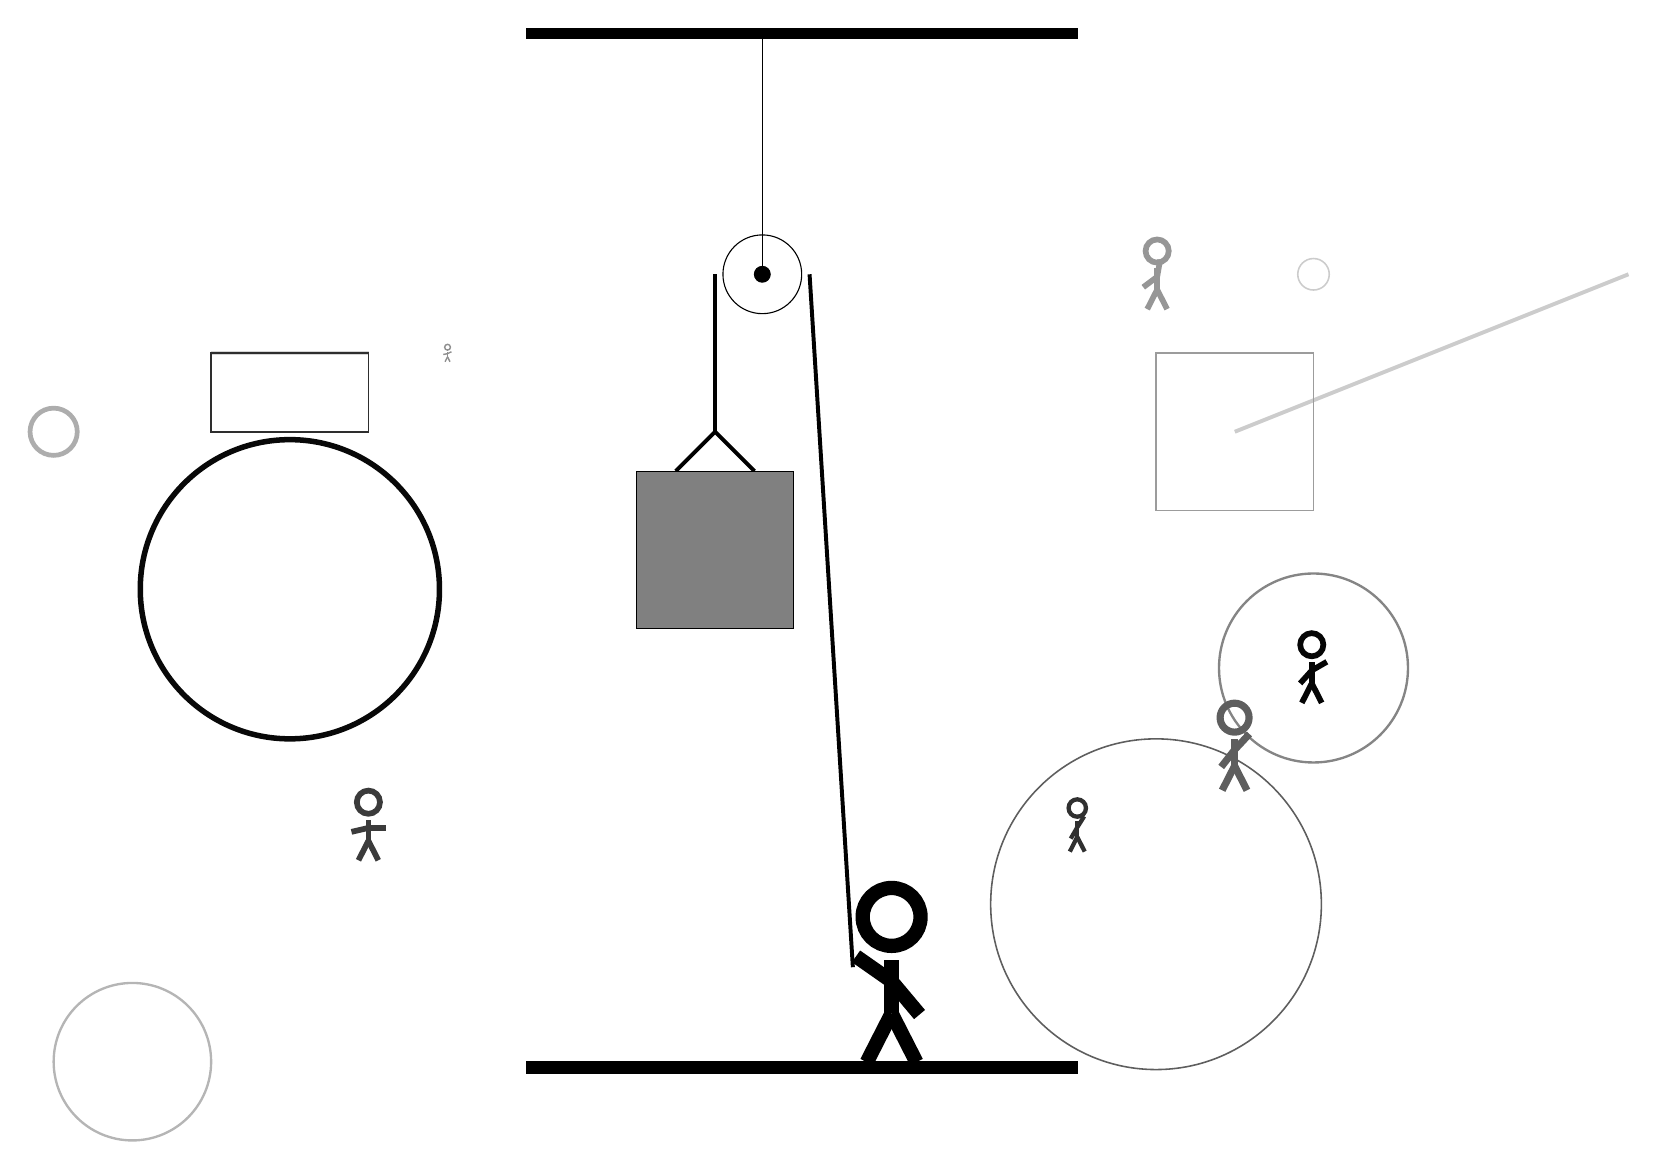
\begin{tikzpicture}
		%%%%% START %%%%%
		
		\draw[fill=black] (-2, 10) rectangle (5, 10.125);
		
		\draw (1, 7) circle (0.5);
		\draw[fill=black] (1, 7) circle (0.1);
		\draw (1, 10) -- (1, 7);
		
		\draw[line width=0.5mm] (-0.1, 4.5) -- (0.4, 5.0) -- (0.9, 4.5);
		\draw[fill=black!50] (-0.6, 4.5) rectangle (1.4, 2.5);
		
		\draw[line width=0.5mm] (0.4, 7) -- (0.4, 5.0);
		\centerarc[line width=0.5mm](1, 7)(0:180:0.6);
		\draw[line width=0.5mm](1.6, 7) -- (2.15, -1.8);
		
		\node at (2.6, -1.9) {\Strichmaxerl[10][-35][-50]};
		
		\draw [line width=0.7mm, color=black!97](-5, 3) circle (1.9);
		
		\draw [line width=0.2mm, color=black!20](8, 7) circle (0.2);
		\draw[line width=0.5mm, color=black!16](-6, 6) -- (-4, 6);
		\draw [line width=0.3mm, color=black!29](-7, -3) circle (1.0);
		\draw [line width=0.3mm, color=black!48](8, 2) circle (1.2);
		
		\draw[line width=0.2mm, color=black!82] (-4, 6) rectangle (-6, 5);
		\node[line width=0.4mm, color=black!81] at (5, 0) {\Strichmaxerl[3][60][58]};
		\draw [line width=0.2mm, color=black!63](6, -1) circle (2.1);
		\node[line width=0.6mm, color=black!41] at (6, 7) {\Strichmaxerl[4][37][80]};
		
		\node[line width=0.7mm, color=black!77] at (-4, 0) {\Strichmaxerl[4][13][0]};
		\node[line width=0.2mm, color=black!98] at (8, 2) {\Strichmaxerl[4][48][30]};
		\draw [line width=0.6mm, color=black!32](-8, 5) circle (0.3);
		\draw[line width=0.5mm, color=black!20](7, 5) -- (12, 7);
		\draw[line width=0.2mm, color=black!39] (6, 4) rectangle (8, 6);
		\node[line width=0.3mm, color=black!44] at (-3, 6) {\Strichmaxerl[1][11][26]};
		\node[line width=0.3mm, color=black!63] at (7, 1) {\Strichmaxerl[5][52][47]};
		
		
		\draw[fill=black] (-2, -3) rectangle (5, -3.15);
		
		%%%%% END %%%%%
	\end{tikzpicture}
\end{document}